\documentclass[a0,portrait,final]{a0poster}

\usepackage{calc}
\usepackage{epsfig}
\usepackage{xspace}
\usepackage{amsmath}
\usepackage{wrapfig}
\usepackage{multirow}
\usepackage{rotating}
\usepackage{arydshln}
\usepackage{booktabs}
\usepackage{multicol}
\usepackage{enumitem}
\usepackage{inconsolata}
\usepackage[english]{babel}
\usepackage{pstricks,pst-grad}
\usepackage{hyperref}
\usepackage{listings}
\usepackage{color}


\newcommand{\tail}[1]{$Q_{tail}${}}
\newcommand{\head}[1]{$Q_{head}${}}
\newcommand{\stail}[1]{$S_{tail}${}}
\newcommand{\shead}[1]{$S_{head}${}}
\newcommand{\etail}[1]{$E_{tail}${}}
\newcommand{\ehead}[1]{$E_{head}${}}


\newrgbcolor{bluisti}{0.02 0.23 0.38}% #073B62 R7 G59 B98
\newrgbcolor{arancioneisti}{0.98 0.44 0.08}% #FC7216 R252 G114 B22
%\newrgbcolor{orangered}{1 0.14 0.00}%orangered rgb(100%, 14%, 0%
%\newrgbcolor{rosso}{0.80 0.00 0.00}%
%\newrgbcolor{yahoo}{0.40 0.00 0.60}%concord grape rgb(40%, 0%, 60%)
%\newrgbcolor{verde}{0.0 0.702 0.0}

\setlength{\columnsep}{1in}
\setlength{\parindent}{0.0cm}

\newcommand{\pbox}[3]{
	\begin{center}
	\psshadowbox[linewidth=2mm,framearc=0.1,framesep=1em,shadowsize=4mm,shadowcolor=lightgray,linecolor=#2]{
		\begin{minipage}[t][][t]{#1}{
			#3 %text
		}\end{minipage}
	}
	\end{center}
}

\newcommand{\dexter}[1]{{\sf Dexter}\xspace}

\newlength\ptitlespace
\setlength\ptitlespace{2.6cm}

\newcommand{\ptitle}[1]{
	\vspace{\ptitlespace}
	\pbox{0.92\columnwidth}{arancioneisti}{
		\begin{center}
		\textsc{\LARGE\bluisti{#1}} %text
		\end{center}
	}
	\vspace{0.5\ptitlespace}
}

\newcommand{\btitle}[1]{\begin{center} \Large{\textsc{#1}} \end{center} \vspace{1.5cm}}
	
\begin{document}
	\newlength\logosize
	\setlength\logosize{8cm}
	\pbox{0.96\textwidth}{arancioneisti}{
	\centering
	\begin{tabular}{ccc}
		\begin{minipage}[c]{\logosize}
		\centering
			
\includegraphics[width=5cm]{img/ucl.eps}
		\end{minipage}
	&
		\begin{minipage}[c]{0.98\textwidth-2\logosize}
		\centering\textsc{}
		\Huge \textsc{Bringing Head Closer to the Tail\\ with Entity Linking}\\[8mm]
	\Large{Manisha Verma$^{1}$, Diego Ceccarelli$^{2,3}$}\\
	\Large{$^1$ UCL Department Of Computer Science}
	\Large{$^2$ ISTI-CNR, Pisa, Italy}\hspace{2cm}\Large{$^3$ IMT Lucca}\\
	
		\end{minipage}
	& 

	\begin{minipage}[c]{\logosize}
	\centering
	
	\end{minipage}
		\begin{minipage}[c]{\logosize}
		\centering
		
\includegraphics[width=9cm]{img/logohpc.eps}
		
\includegraphics[width=5cm]{img/logoisti.eps}
		\end{minipage}
	\end{tabular}
	}


\vfill
\large


\begin{multicols}{2}
\ptitle{Introduction}
	Search queries follow a \emph{Zipfian} distribution.
	 
	\begin{itemize}
	 
	 \item \textbf{\emph{Head queries}: }Few popular queries with a large volume.
	 \item \textbf{\emph{Tail queries}: }A significant percentage of queries that occur rarely. 
	

	\end {itemize}	
	\vspace{10mm}
	\begin{center}
	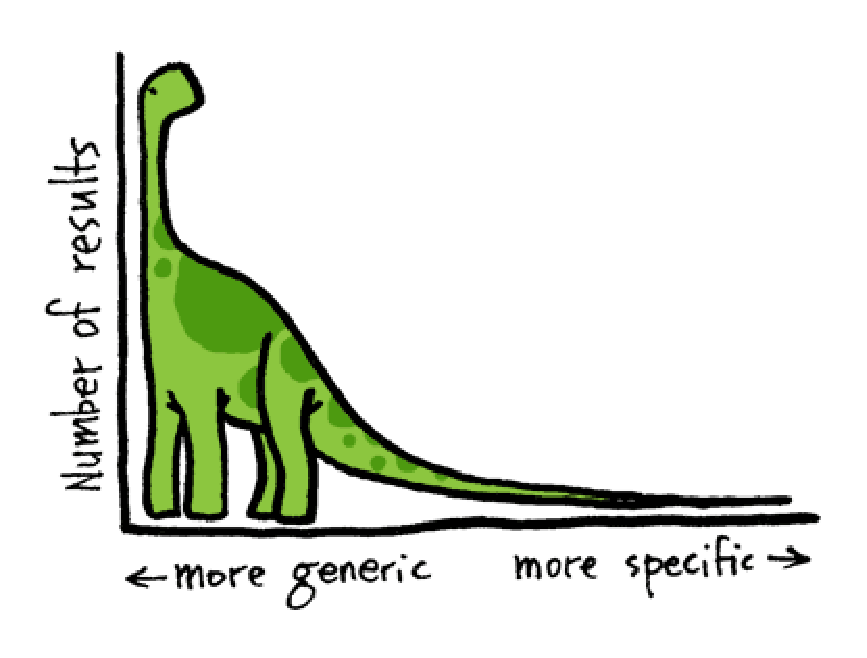
\includegraphics[width=0.9\columnwidth]{img/long-tail.eps}
	\end{center}
	 	 
	Given a search log, there is \textbf{\color{blue}sufficient data} to analyze \textbf{\color{blue}head queries} 
	but \textbf{\color{red}insufficient data (low frequency, limited clicks)} to draw any conclusions 
	about \textbf{\color{red}tail queries}. 
	
	\begin{itemize}
	
	\item Knowledge bases have enabled understanding of short or long unstructured text. 
	
	\item Can we quantifying the extent of \textbf{overlap between long tail and head queries} 
	by means of \textbf{entity linking}.
	
	\end{itemize}
	
 \ptitle{Research Questions}
  
	  \begin{itemize}
		\LARGE 
	  	\item Are tail queries a different means to inquire about entities mentioned in the head queries? 
	  	\item Can we find tail queries about entities that are not searched in the head (\emph{tail entities})?
	  	\item Can we find a relationship between \emph{tail entities} and \emph{head entities}?  
	  \end{itemize}
	
	 %We specifically analyze the frequency distribution of entities in head and tail queries. 
	
\ptitle{Entity Linking Problem}

%The entity linking task aims at identifying, given a plain document, the small fragments of text (interchangeably called \emph{mentions} or \emph{spots}) referring to any \emph{named entity} that is listed in a given knowledge base, e.g. Wikipedia. The ambiguity of natural language makes it a non trivial task. The same entity can be in fact mentioned with different text fragments, e.g., ``President Kennedy'' or ``John F. Kennedy''. On the other hand, the same mention may refer to different entities, e.g., ``Michael Collins'' may refer to either the well known astronaut, or to the Irish leader and president of the Irish provisional government in 1922.

The annotation is usually organized in three subtasks:
\begin{enumerate}
	\item \textbf{Spotting}: discover the fragments that could refer to an entity. A set of candidate mentions is detected, and for each mention a list of candidate entities is produces;
	\item \textbf{Disambiguation}: for each spot associated with more than one candidate, a single entity is selected to be linked to the spot;
	\item \textbf{Ranking}: the list of entites detected is ranked according to some policy, e.g. annotation confidence. 
\end{enumerate}

Our entity linker Dexter (\url{dxtr.it}) identifies 
at least one spot in $13,977$ ($70\%$) and $4,901,987$ ($63\%$) \head{} and \tail{} 
respectively.

\vspace{5mm}
\begin{center}
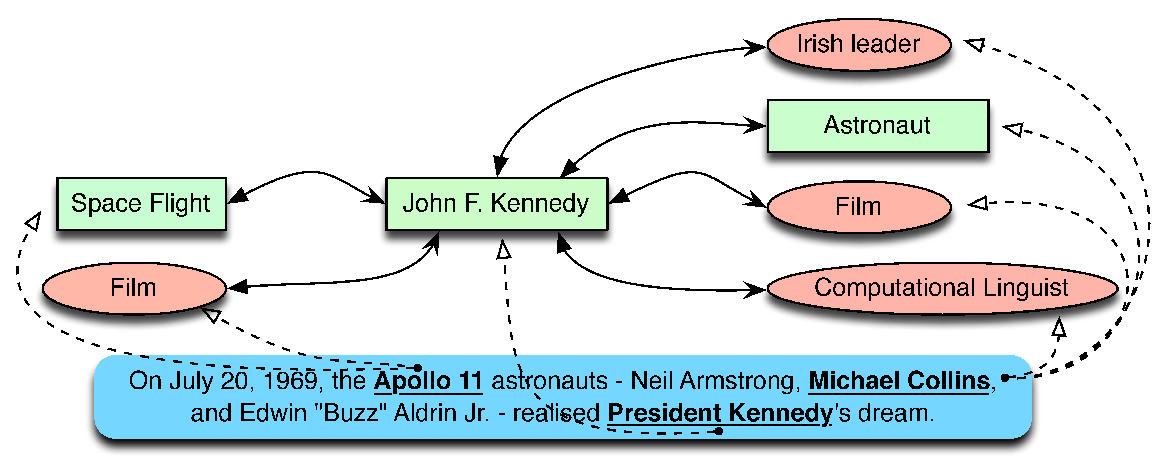
\includegraphics[width=0.92\columnwidth]{img/annotation-example.eps}
\end{center}
%Some real query examples with annotations are:
\begin{itemize}
\item \fbox{\textbf{first citizens bank} and trust \textbf{Raleigh NC}} contains
\texttt{Raleigh,\_North\_Carolina} and \texttt{First\_Citizens\_Bank};
% \item \fbox{\textbf{internal revenue service} de \textbf{puerto roco}} is annotated with the entities \texttt{Roco} and
% \texttt{Internal\_Revenue\_Service};
\item \fbox{\textbf{Tennessee walking horses} in \textbf{Missouri}} is annotated
with \texttt{Missouri} and  \texttt{Tennessee\_Walking\_Horse};
\item \fbox{\textbf{i love you} \textbf{remix} featuring \textbf{Jim Jones} and
\textbf{black rob}} contains  \texttt{I\_Love\_You,\_Man},
\texttt{Remix}, \texttt{Jim\_Jones\_(rapper)}, \texttt{Black\_Rob}.
 \end{itemize}


\ptitle{Analysis}

AOL log consists of approximately 20 million queries submitted by $650,000$ users. There are in total $10,154,742$ distinct queries. 
We extract 2 distinct sets from these queries: 
\begin{description}
	\item{\textbf{\tail{}}} Tail queries with frequency \emph{lower than or equal} to $2$. Contains $7,746,607$ distinct queries, i.e. $76\%$ of distinct queries. %, but it is $26\%$ of the total volume of the queries.
	\item{\textbf{\head{}}} Head queries with frequency \emph{greater than} $99$. The set contains $19,953$ distinct queries, i.e. $0.002\%$. % if we look at the distinct queries, these queries represent $26\%$ of total query volume.
\end{description}
Although, the two sets differ in number of queries ($\sim19$K versus $\sim7$M), they \textbf{cover the same fraction of total queries issued} to the search engine. %All our analysis are performed on these two sets.


\begin {itemize}

	\item {\textbf{Spot-Entity Distribution}:} While queries in head and tail follow totally different distributions, when we 		look at their spots/entities, the distributions are similar as shown in Figure \ref{img:distributions}.  
		\vspace{10mm}
		\begin{center}
		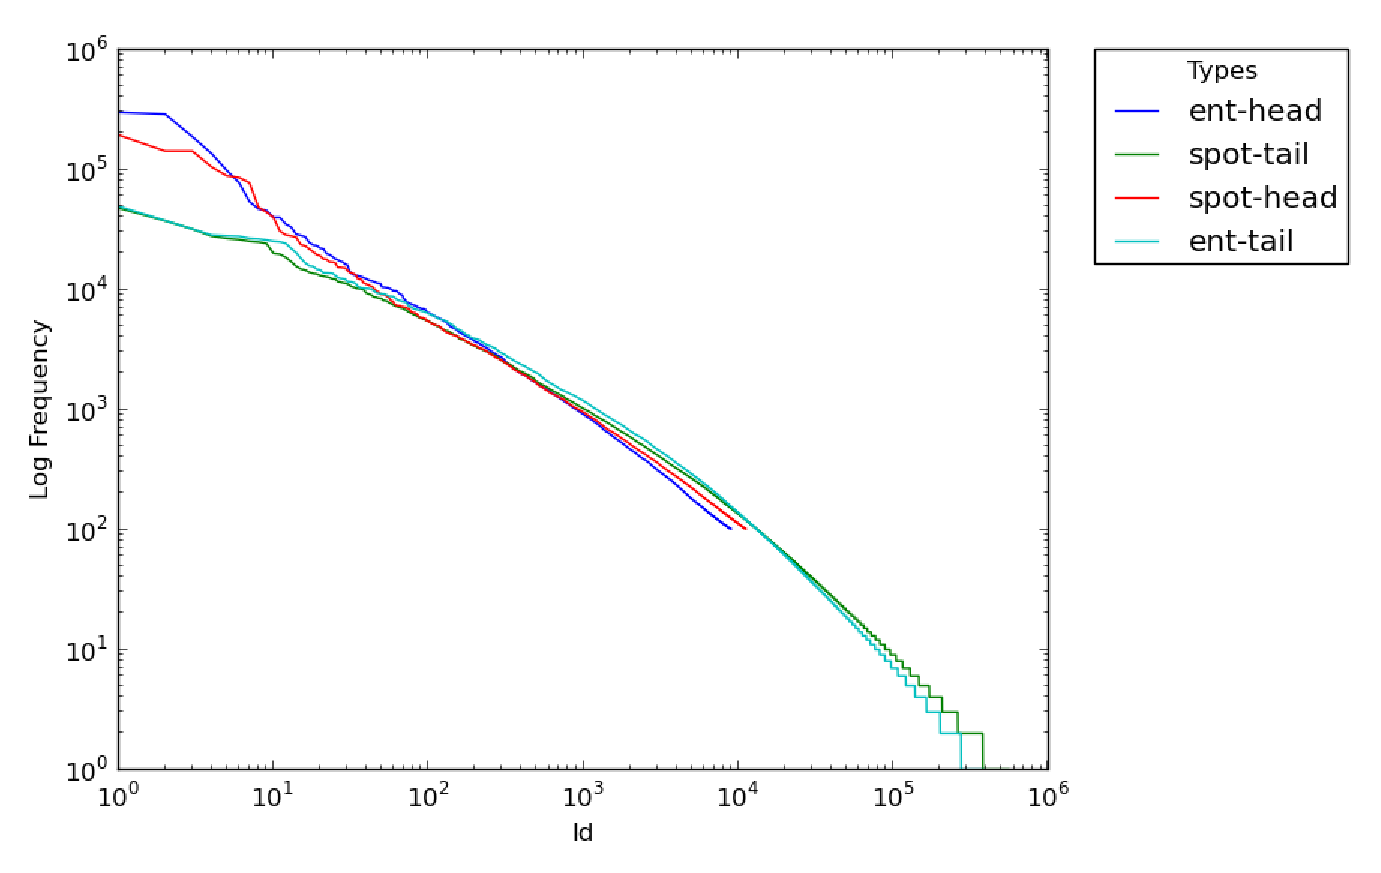
\includegraphics[width=0.6\columnwidth]{img/head-tail-ent-spot-dist.eps}
		%\caption{Frequency distributions for spots and entities in \head{} (spot-head, ent-head) and \tail{} (spot-tail, ent-tail)}
		\label{img:distributions}
		\end{center}

	\item {\textbf{Popular Head and Tail Entities Overlap}:} On sorting the entities based on their frequency in \head{} 		and \tail{} respectively and comparing the ranked lists at different cutoffs, Jaccard distance between the ranked lists is 		0.25 at 5000. At smaller cutoffs (top 50 entities) the Jaccard is 0.05. 
	
\begin{tabular}{lc|lc|lc|lc}
\toprule
\multicolumn{4}{c}{\head{}} & \multicolumn{4}{c}{\tail{}}\\
\multicolumn{2}{c}{\shead{}} & \multicolumn{2}{c}{\ehead{}} & \multicolumn{2}{c}{\stail{}} & \multicolumn{2}{c}{\etail{}}\\
\midrule
google         & 342,602  &  Google  		   & 349,337  &  florida 	 &	47,718	&	Florida 		& 49,366 \\
myspace        & 194,093  &  Yahoo\!  		   & 299,718  &  texas  	 &	 37,388  &   Texas   		& 37,526 \\
yahoo          & 142,361  &  Myspace 		   & 289,353  &  ohio    	 &	31,861   &   Ohio    		& 31,905 \\			
ebay           & 142,257  &   EBay   		   & 187,633  &  edu     	 &	26,641   &   New\_York        & 28,396 \\
yahoo.com      & 104,696  &  MapQuest          & 135,179  &  state   	 &	26,066   &   .edu    		& 26,642 \\
mapquest       & 88,617   &  Google\_Search     & 98,112   &  california  &   25,233  &   U.S.\_state      & 26,392 \\
google com     & 85,670   &  Hotmail           & 53,925   &  new york    &   24,865  &   California      & 25,859 \\
my space       & 48,401   &	  Bank\_of\_America  & 46,922   &  hotel   	 &	20,018   &   Real\_estate     & 25,232 \\
www.yahoo.com  & 44,198   &  Craigslist        & 45,586   &  real estate &   19,702  &   Myspace 		& 24,998 \\
internet       & 39,865   &  Ask.com           & 39,873   &  myspace 	 &	18,533   &   Floruit 		& 24,207 \\
ebay com       & 30,652   &  Internet          & 39,865   &  restaurant  &  17,065   &   Restaurant      & 21,996 \\
hotmail.com    & 28,492   &  Pornography       & 35,089   &  michigan    &   15,635  &   Hotel   		& 20,289 \\
map quest      & 27,949   &  Tattoo            & 33,113   &  new jersey  &   14,813  &   Nudity  		& 18,245 \\
craigslist     & 27,222   &  American\_Idol     & 28,890   &  georgia 	 &	14,525   &   United\_States   & 16,680 \\
american idol  & 23,665   &  Yahoo!\_Mail       & 28,238   &  black   	 &	13,921   &   Michigan        & 15,763 \\
\bottomrule
\end{tabular}

	\item {\textbf{Queries with Multiple Entities}:} There are several queries in the log with multiple entities. 
	On average tail queries have more entities than head. \textbf{Do tail queries inquire about entities in the head?} The percentage of 		tail queries containing only head entities, only tail entities ($\in$ \etail{} $\setminus$ \ehead{}) or both is shown in 		Figure \ref{img:headTailEntPercent}.
	
	%\begin{figure}	
	%\begin{subfigure}
	
	%\end{subfigure}
		
	%\begin{subfigure}
		\vspace{10mm}
		\begin{center}
		%\centering
		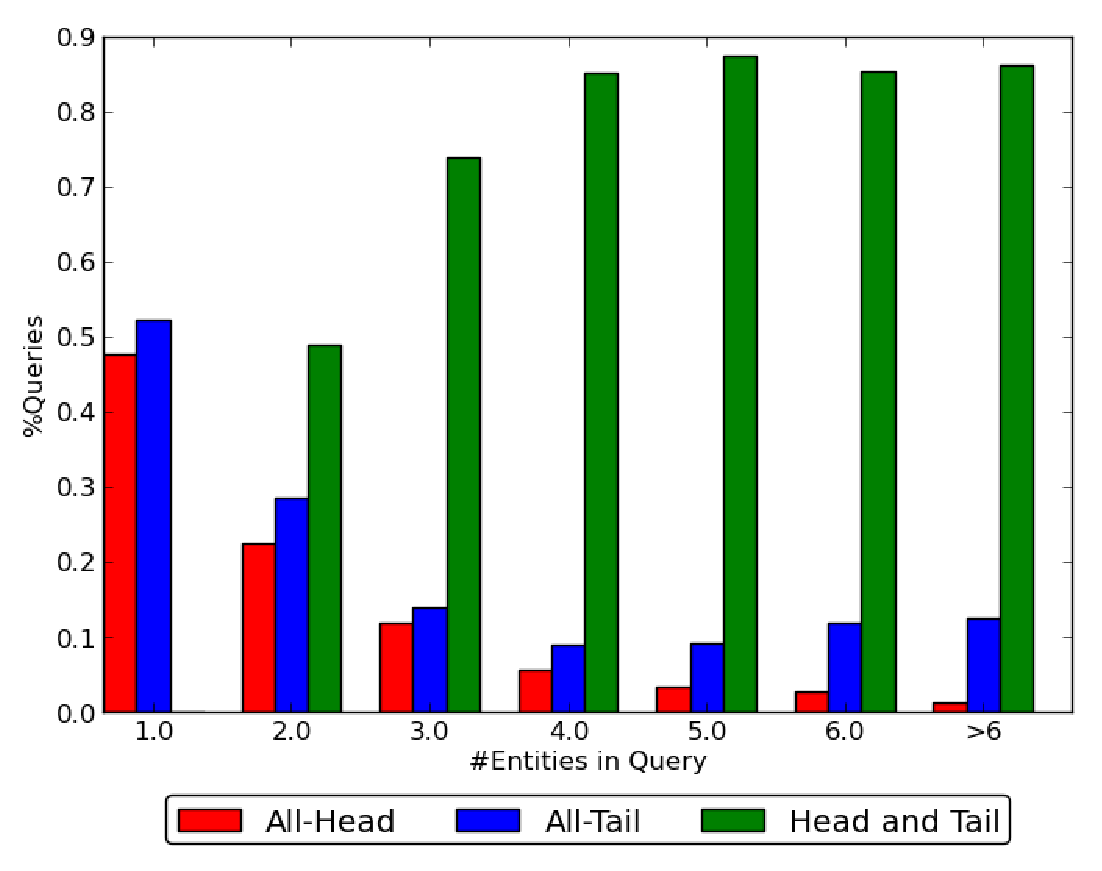
\includegraphics[width=0.5\columnwidth]{img/entity-head-tail-count.eps}
		%\caption{Percentage of tail queries with only head, only tail or both entities}
		\label{img:headTailEntPercent}
		\end{center}
	%\end{subfigure}
	%\end{figure}
\end {itemize}



\end{multicols}
\vfill
\centering
\begin{minipage}[c]{\textwidth}
\rule{\textwidth}{1pt}
\textit{ESAIR '14  -- 7$^\textit{th}$ International Workshop on Exploiting Semantic Annotations in Information Retrieval. November 7, 2014. Shanghai, China.}
%\textit{ESAIR '14  -- The 23\emph{rd} ACM Conference on Information \& Knowledge Management. November 3-7, 2014. Shanghai, China}
\end{minipage}

\end{document}
